% $Author$ $Date$
%
% Predrag created file siminos/CLE/flotsam.tex      Dec 20 2009

\section{Flotsam}

This chapter contains material which has not been included in
publication
{\tt siminos/CLE/CLE.tex}.

{\bf ES 2009-12-22:}

I find the following notion of global vs local reasonable but it contradicts
the usage of local in the text, especially in comparison of invariant polynomials
to \mframes\ and \slice s. Here by \emph{global} method we mean
one which permits reducing dynamics to return maps associated with a finite set
of \Poincare\ sections, while a \emph{local}
method is one that is specific to a solution, even if the latter is a global object such as a periodic
orbit.




{\bf ES 2009-12-19 replaced:}
 On the other hand when one faces
nonlinear field theories\rf{chfield}, either classical or
quantum, the identification existense of order and organization
identified within the bewildering wealth of solutions. Dynamics
within the chaotic attractor of a low-dimensional, continuous
time, (state-space-)volume contracting flow can be in many
cases\rf{gilmore2003} understood by reduction to a discrete time map within a
Poincar\'e section. For sufficiently strong volume contraction
such a mapping provides a complete topological characterization
of the attractor\rf{gilmore2003}. Moreover the set of compact
invariant solutions, equilibria and periodic orbits, organize
the dynamics around them.

{\bf ES 2009-12-19 dropped: }
Nevertheless, many of the early examples of chaotic attractors where
observed in very drastic truncations of PDEs, such as the Lorenz flow\rf{lorenz}.

, see, for example,
Cushman and Bates\rf{CushBat97} or Marsden and Ratiu\rf{MarsdRat94}


{\bf ES 2009-12-20 dropped}, not sure it is true and does not offer to the discussion:

When one takes syzygies into account in rewriting the
dynamical system, singularities are introduced. For instance
if we solve \refeq{eq:syzLaser} for $u_2$ and substitute into \refeq{eq:CLEip}
the latter reads
\beq
\begin{split}
  \dot{u}_1 &=2\,\sigma\,(u_4-u_1)\,,\\
  \dot{u}_2 &=-2\left(\,\frac{u_3^2+u_4^2}{u_1} - \rho_2\, u_3 -\,(\rho_1-u_5)\,u_4\right)\,,\\
  \dot{u}_3 &=-(\sigma\, +1)\,u_3+\rho_2\, u_1+e\, u_4\,,\\
  \dot{u}_4 &=-(\sigma\, +1)\,u_4+\,(\rho_1-u_5)\,u_1+\sigma\, \frac{u_3^2+u_4^2}{u_1}-e\,u_3\,,\\
  \dot{u}_5 &=u_4-b\, u_5\,
\end{split}
\label{eq:CLEipSyz}
\eeq
clearly singular as $u_2\rightarrow 0$.

{\bf PC 2010-01-25 dropped:}


As we will see in \refsect{s:StabReq}, \REQV{}{1} of {\cLe}
for the parameter set we study here is unstable with one
complex expanding eigenvalue. Yet, being a periodic orbit,
its unstable manifold is three-dimensional, with one
eigendirection corresponding to the direction of $\vf$ which
also coincides with the direction of rotations of the system.
In \reffig{fig:CLE} we plot one trajectory on the unstable
manifold of \REQV{}{1}. While it spirals away from
$\REQV{}{1}$ it also ``drifts'' along the direction of
rotations of the system. This drifting motion obscures
understanding of the stretching mechanism along the expanding
eigendirection and subsequently the folding of the unstable
manifold back to itself.


{\bf ES 2009-12-21 redundant/replaced:}
In {\cLe} a secondary
bifurcation from \REQV{}{1} is expected, according to Krupa's
theorem\rf{Krupa90}, to result in \emph{relative periodic
orbits} that satisfy
\beq
	\LGelement{l_p}x(t+T_p)=x(t)\,,
\eeq
{\ie} they ``return'' after a time period $T_p$ to a point
that maps to the initial one under a group transformation
$\LGelement{l_p}$ with group parameter period $l_p$. A {\rpo}

{\bf ES 2009-12-21 dropped:}

rephrased: To cite Fels and Olver\rf{FelsOlver98}:
moving frames where ``first introduced by Gaston Darboux
and brought to maturity by \'Elie Cartan.''


{\bf ES 2009-12-21 dropped:}

We have noted that \SOn{2} acts regularly and freely on
$X^*=\Rls{5}\backslash\{x_1=x_2=y_1=y_2=0\}$ and thus we are
guaranteed to find the fundamental invariants by the method
of moving frames if we restrict attention to $X^*$.


Here we can use the fact that
$- \ssp \cdot \Lg\cdot\Lg \cdot \slicep
 = (\ssp \cdot \slicep )_4 =
    x_1 x_1^{*}
   +x_2 x_2^{*}
   +y_1 y_1^{*}
   +y_2 y_2^{*}
$
is the dot-product restricted to the 4-dimensional
representation of $\SOn{2}$.

A generic  $ \slicep $ can be brought to form $ \slicep  =
(0,1,y_1^{*},y_2^{*})$ by a rotation and rescaling. Then $\Lg
\cdot \slicep   = (1,0,y_2^{*},-y_1^{*})$, and
\beq
\frac{(\vel \cdot \Lg \cdot \slicep )}{(\ssp \cdot\slicep )_4} =
\frac{\vel_1 + \vel_3 y^{*}_2 -\vel_4 y^{*}_1}
     {x_2 + y_1 y^{*}_1 + y_2 y^{*}_2}
%\frac{\vel_1 x^{*}_2 -\vel_2 x^{*}_1 + \vel_3 y^{*}_2 -\vel_4 y^{*}_1}
%     {\vel_1 x^{*}_1 + \vel_2 x^{*}_2 + \vel_3 y^{*}_1 + \vel_4 y^{*}_2}
\,.
\label{PCsectSin}
\eeq


 {\bf ES 2009-12-21 dropped (and PC agrees):}

We say that $\Group$ acts locally freely on \pS\ if for any
$\ssp\in\pS$ the isotropy subgroup $\stab{\ssp}$ is a
discrete subgroups of $\Group$. An r-dimensional compact Lie
group $\Group$ acts \emph{locally freely} on $\pS$ if and
only if it has $r-dimensional$ orbits\rf{FelsOlver99}. A
group $\Group$ acts freely on $\pS$ if all isotropy subgroups
are trivial: \stab{\ssp}=\{e\} for all $\ssp\in \Manif$. If
in addition for each point $\ssp\in \Manif$ there exists an
arbitrarily small neighborhood $U$ such that each orbit of
$\Group$ intersects $U$ in a pathwise connected subset, then
the group acts regularly.

{\bf ES 2009-12-21 dropped:}

A group $\Group$ acts semi-regularly on $\pS$ if all its
orbits have the same dimension. Therefore the group orbits of
a group that acts semi-regularly foliate $\pS$. A sufficient
condition for a semi-regular action is that for any
$\ssp\in\pS$ the isotropy subgroup $\stab{\ssp}$ is a
discrete subgroup of $\Group$. If a Lie group $\Group$ acts
semi-regularly on a manifold $\Manif$,

Note that locally free action implies semi-regular action.

{\bf ES 2010-01-22 dropped:}

In this section we present the {\mframes}, introduced by G. Darboux and
systematized by \'E. Cartan\rf{CartanMF}.
Fels and Olver\rf{FelsOlver98,FelsOlver99} reformulated the method so that a
moving frame is simply an equivariant mapping from the space on which a
group acts to the group parameter.  In \refsect{s:mfReqb} we will
exploit the geometric interpretation of moving frames for a more direct and
efficient approach to symmetry reduction. \refrefs{FelsOlver98,FelsOlver99}

A moving frame is a smooth
$\Group$-equivariant mapping $\rho$ from $\Manif$ to the
$\Group$, that is to the group parameters. \ES{perharps not
needed: One distinguishes between left moving frames for which
the equivariance condition is $\rho(\LieEl x)=\LieEl\rho(x)\,,\
x\in\Manif\,,\ \LieEl\in\Group$ and right moving frames for
which the equivariance condition is $\rho(\LieEl
x)=\rho(x)\LieEl^{-1}\,,\ x\in\Manif\,,\ \LieEl\in\Group$.  As shown in \refref{FelsOlver99} a moving frame exists
in a neighborhood of a point $x\in\Manif$ if and only if
$\Group$ acts freely and regularly near x.} For the practical
construction of a moving frame for an $N-$dimensional Lie group
$\Group$ we will need to define a slice.
Therefore the existense of a moving frame depends on
group orbits having the same dimension.

re-insert?: To construct a moving frame, let $K\subset\Manif$ be a {\slice}. For $x\in \Manif$, let
$\LieEl=\rho(x)$ be the unique group element that maps $x$
to the {\slice}: $g x = \rho(x) x\, \in K$. Then
$\rho:\Manif\rightarrow \Group$ is a right moving frame\rf{FelsOlver98}.

A {\slice} $K$ can be defined by means of level sets of
functions $K_i(x)=c_i$, where $x\in V$ and $i=1,\ldots,r$. If
the $K_i(x)$ coincide with the local coordinates $x_i$ on the
manifold $V$, \ie~$K_i(x)=x_i$,

{\bf ES:Moved example from movingFrames.tex here, some bits should still be rescued:}

In this section we illustrate symmetry reduction through
the use of invariants computed
with the moving frame method in the example of \cLe.
The $z$-axis is the \fixedsp\ of \SOn{2} acting by
\refeq{eq:SO2act} on \Rls{5}. Therefore we can define
a coordinate {\slice} on $\Rls{5}\backslash\{x_1=x_2=y_1=y_2=0\}$
by, for instance,
\beq%\label{eq:CLEsliceSO2}
x_1=0,\,x_2>0\,.
\eeq
We can now construct a moving frame for the action
\refeq{eq:SO2act} of $\SOn{2}$ as follows. We write out
explicitly the group transformations:
\begin{subequations}%\label{eq:CLEnorm}
\begin{align}
 	\overline{x}_1 &= x_1 \cos\theta - x_2 \sin\theta\cont
	\overline{x}_2 &= x_1 \sin\theta + x_2 \cos\theta\cont
	\overline{y}_1 &= y_1 \cos\theta - y_2 \sin\theta\cont
	\overline{y}_2 &= y_1 \sin\theta + y_2 \cos\theta\cont	
	\overline{z} &= z\,.
\end{align}
\end{subequations}
We set $\overline{x}_1=0$ and solve
\refeq{eq:CLEexplSO2a} for the group parameter to obtain the moving frame
\beq
	\theta=\tan^{-1}\frac{x_1}{x_2}
% 	\label{eq:CLEmf}
\eeq
which brings any point  back to the {\slice}.
Here it is important that
$\tan^{-1}$ distinguishes quadrants in the $(x_1,x_2)$ plane to ensure that the
transformation results in the correct geometric
interpretation, \ie\ to ensure $x_2>0$.
Substituting \refeq{eq:CLEmf} in the remaining equations \refeq{eq:CLEnorm} we
get the invariants
\beq
\begin{split}
	\overline{x}_2 &=  r_1 = \sqrt{x_1^2+x_2^2} \cont
	\overline{y}_1 &= {(x_2 y_1-x_1 y_2)}/{r_1}\cont
	\overline{y}_2 &= {(x_1 y_1+x_2 y_2)}/{r_1}\cont	
	\overline{z} &= z\,.
% 	\label{eq:invLaser}
\end{split}
\eeq
    \ES{The solution $\theta = 2
    \tan^{-1}\frac{-x_2+\sqrt{x_1^2+x_2^2}}{x_1}$ was
    returned by Mathematica. If we use $\theta =
    \tan^{-1}\frac{x_2}{x_1}$ without taking care of the
    quadrant our results are multiplied by $sgn(x_2)$.}


{\bf ES: I will need to rewrite the following}

In terms of projecting dynamics
on variables \refeq{eq:invLaser} (or applying the equivalent
procedure of rotating points back to the \slice) this means that
we need to take into account the direction along which
we approach zero and use the `angle
of descent' as the angle with which we rotate points back to the \slice, if such
points have exactly $x=0$.

Note that the invariants are not defined on
the subspace $U_S$ defined by $x_1=x_2=0$ even though the
group action is non-regular only in a subset of $U_S$, the
$z$-axis $x_1=x_2=y_1=y_2=0$ which is the \fixedsp\ of \SOn{2}.
In the spirit of \refref{GL-Gil07b} the transformations \refeq{eq:invLaser}
can therefore be characterized as non-optimal, in the sense
that we have singularity in a proper superset of $\Fix{\SOn{2}}$.
    \PC{``proper superset''? Il cano no parla questa lingua}
The reason the transformations fail on $U_S$ and not only on the $z$-axis
can be traced back to the way we construct the moving frame. The action
of the group can be thought of as a direct sum of irreducible
actions and the corresponding invariant (linearly irreducible)
subspaces are the $(x_1,\,x_2)$ and $(y_1,\,y_2)$
planes.
%PC OK \ES{Not sure if planes is acceptable term here.}.
Since irreducible subspaces are by definition group-invariant
implies that we could define a moving frame in any one of them
independently. The singular subspace would then be determined
by the fixed points of group action in this subspace alone.
For instance, by choosing an angle in the $(x_1,\,x_2)$ irreducible subspace
as the moving frame map, the singular set is the point
$x_1=x_2=0$ in this irreducible subspace. Going back to the full
$5$-dimensional space the singular set of the transformations
is still given by $x_1=x_2=0$.
%}

While a singularity in $\Fix{\SOn{2}}$ cannot be reached by generic orbits
as {\fixedsp s} are flow invariant, the same is not true for {\fixedsp s}
of irreducible representations of the group action\ES{make sure!!!}.
The fact that trajectories of \cLf\ in \reffig{fig:CLEmf} stay away from $r_1=0$ is therefore
fortuitous.

{bf ES dropped, not true.}

We see that the problems of
\reffig{fig:CLEmf} are not present in \reffig{fig:CLEmfReqb1}, since
the slice now is not defined only where the group action is not free,
that is in the set of points that are fixed by the group action. This
is the $z$-axis and as we have remarked it cannot be reached by generic
trajectories. We have to caution the reader that this is a fortuitous
event. For more general group representations symmetry reduction through
the use of a slice will be at best local as we intend to discuss
elsewhere\rf{SCD09b}. Nevertheless, using local slices defined by \refeq{PCsectQ}
to tesselate the \reducedsp\ is an optimal choice in the sense that any
failure will occur in \fixedsp\ $\Fix{\LieElrep_a}$ of some subgroup
$\LieElrep_a$.




{bf ES dropped old conclusions.}

Implementing symmetry reduction in any of the above ways, the
reward is the same: The dynamics are reduced to a return map
to the Poincar\'e section, which due to the very strong
contraction is approximately $1$-dimensional. The dynamics on
the Poincar\'e section are parametrized by the Euclidean
distance of points along the unstable manifold, as we did for
the Lorenz example. The return map is unimodal and allows for
systematic determination of all cycles of a given length.
Here we were able to determine all cycles up to length $7$,
using the return map of \reffig{fig:CLEinvRM} to generate
guesses, and the multiple-shooting algorithm\ES{reference.}
to refine them to machine accuracy.

We have presented symmetry reduction of \cLe\ dynamics through the use of
(a) a Hilbert basis,  (b) invariants generated by the {\mframes},
(c) a combination of use of a Poincar\'e section and a slice and (d) through
the infinitesimal application of a moving frame map, termed the method of
slices. We observe that with the exception of the Hilbert basis method all
approaches are local in nature and essentially interrelated. The Hilbert basis
method unfortunately does not scale well with state-space and group dimension
and therefore cannot be used in high-dimensional problems.

In both the finite and infinitesimal time formulation of a moving frame map
we might understand the singularities through the analogy between a slice
and a Poincar\'e section. In symmetry reduction singularities
are introduced at points in space that are fixed under the group action.
Fixed points of time evolution are atypical and do not lie on a Poincar\'e section
unless the section has been specifically chosen so that it contains them.
Therefore one cannot expect, for a flow with many fixed points, to
get away with using just a single Poincar\'e section. The same is
true for fixed points of group actions and their generalization, \fixedsp.
One cannot expect to use a single \slice\ to cover different \fixedsp s
of continuous (sub)groups.

{\bf PCS 2010-01-26} dropped:
    so we assume $\Group$ is a compact Lie group.
    Any compact Lie group $\Group$ acting on $\Rls{d}$ is
    a subgroup of $\On{d}$, \cf\ for example \refref{golubII}.



As the systems that we study here are not associated with a
variational principle, Noether's theorem does not
apply, and in general no conserved
quantities are associated with continuous symmetries of
such systems.
    \PC{include discussion, references from the blog here.}

``
Such a conserved quantity would restrict dynamical
trajectories to an invariant manifold locally transverse to
the direction of group action. In the contrary here the
system also evolves along the direction of group action.
    ''

{\bf PC 2010-01-27}
Being on a constant energy surface does not mean we do
not evolve in time, for example.
{\bf ES:} You are right, this statement is not correct in
general. What I had in mind was cases such as
conservation of angular momentum in central force 		
problems fixes the plane of motion.

{\bf PCS 2010-01-26} dropped:
The stratification
of $\pS$ induced by the group action is carried over to
the quotient space with each disconnected set in a stratum
mapped to the same manifold in quotient space. Yet, a
fundamental problem with symmetry reduction is that the orbit
space is in general not a manifold. Unless the action of the
group is free, group orbits do not have the same dimension
and different strata are mapped to manifolds of different
dimension. We will see this property of quotient space
manifest itself in different ways depending on the reduction
method but always introducing some singularity even though
there is nothing singular about $\pS$ or the flow of the
dynamical system on it.
        \ES{Either define stratum, or simplify the discussion
		here.}



{\bf ES} In thesis and here Hilbert
polynomials are used as an introduction to this use of moving
frames. It used to be more important in previous versions.

{\bf PC 2010-01-26:}
   The problem with giving Krupa the credit is that he is
   generalizing bifurcation from a fixed point to a Hopf
   cycle, ie., he has a 'quasi-periodic modulated traveling' wave in mind.
   Our \rpo's arise from stretching and folding, nor from a
   bifurcation.

{\bf ES dropped: }
I am not sure it is correct for multiparameter groups. Even
for \cLe\ it seems to imply that the slice exists on the $z$-axis,
which I think is not true: The
invariant subspaces are always within the \slice, as $\Lg_a
 \ssp =0$ for $\ssp$ in an invariant subspace.

{bf ES removed, we have said this already but we can merge it
with introductory text:}

The equivalence classes $\Group \, \ssp = \{  \LieEl \, \ssp
| \LieEl \in \Group \}$ are manifolds called the group
orbits. We have thus replaced the dynamical system
$\{\pS,f\}$ by a reduced system $\{\bar{\pS},\bar{f}\}$ where
each  group orbit is a point in the \reducedsp\
$\bar{\pS}=\pS/\Group$.

% Vaggelis                                  Aug 12 2009
%           \refeq{EqMotionMovFramePC} is correct
%           there are problems with the derivation.


{\bf PC 2010-01-26} dropped {\bf ES: } comment:

In equivariance condition \refeq{eq:equivFinite} the group
element $\LieEl$ is time-independent. The condition
corresponds to a ``rigid rotation'' of all points on the
trajectory. In the decomposition $\ssp(t)=
\LieEl(t)\,\sspRed(t)$ you have to invoke some slice theorem
that guarantees existence of such a decomposition locally, as
long as the group action is semi-regular and a slice can be
defined.
\\
{\bf PC 2010-01-26:} this is a recurrent comment that I do
not understand. It's perfectly  OK that $\LieEl= e$, or
$\LieEl \in \Subgroup$, what is the problem of ``guaranteeing
existence of such a decomposition?''

{\bf ES 2010-01-26:}
I use $Q_1$ and $E_0$ for \reqv\ and \eqv\ of cLe and it
would be easier for me to keep it this way in the paper since
otherwise I have to change all figures. I've been using
$\setminus REQB$ and $\setminus EQB$ macros for this. I have
now also redefined $\setminus REQV$ and $\setminus EQV$ macro
so that all text is uniform. Let me know what you prefer.

{\bf PC 2010-01-26:} I think this is a good convention.

{\bf ES 2010-01-27, dropped:}
Geometrically we can interpret the jumps in the
$\overline{y}$ coordinates as follows: We have chosen to
measure angle on one of the irreducible subspaces of \SOn{2},
the $x$-plane, and project the dynamics on orbit space by
counter-rotating in both irreducible subspaces (the $x$- and
$y$-plane.) As long as a trajectory traces one lobe of the
Lorenz attractor the angle varies slowly and no problem
occurs. When a trajectory changes quadrant in the $x$-plane
to visit the almost opposite lobe (due to detuning we do not
visit the lobe related by rotation by $\pi$, in reality no
such thing exists) we get a rapid change in angle as the
trajectory passes close to the origin. In the $y$-plane we do
not necessarily change quadrant. Call $\Delta \theta_x$ and
$\Delta\theta_y$ the change in angle in the $x$- and
$y$-plane respectively, when the trajectory changes quadrant
in the $x$ plane. We always reduce to \reducedsp\ by
correcting by $-\Delta\theta_x$ instead of correcting by the
smallest angle.

{\bf ES 2010-01-27 dropped:}
so that \refeq{cLeMF}, when substituted back to
representation \refeq{CLfRots} of \SOn{2} results to the
correct geometric operation of mapping points back to the
slice. Therefore the range of $\tan^{-1}$ here is
$-\pi<\theta\leq\pi$.

{\bf ES 2010-01-27 merged with existing intro:}

The notion of a {\em moving frame} as a map from a manifold
to a Lie group was introduced by Cartan\rf{CartanMF}. Fels
and Olver view the method as an alternative to the Gr\"obner
bases methods for computing Hilbert polynomials, to compute
functionally independent fundamental invariant bases for
general group actions (with no explicit connection to
dynamics, differential equations or symmetry reduction).
`Fundamental' here means that they can be used to generate
all other invariants. Olver's monograph\rf{OlverInv} is
pedagogical, but does not describe the original Cartan's
method. Fels and Olver papers\rf{FelsOlver98,FelsOlver99} are
lengthy and technical. They refer to Cartan's method as
method of `moving frames' and view it as a special and less
rigorous case of their `moving coframe' method. The name
`moving coframes' arises through the use of Maurer-Cartan
form which is a coframe on the Lie group $\Group$, \ie, they
form a pointwise basis for the cotangent space.

{\bf ES 2010-01-07:}
define $\groupTan$ in symmetry section, choose a prettier
symbol. I see it coming; you will make it all look Greek to
me. {\bf ES:} Well, unless 	you want to change time to $\tau$
we have to change 	group tangent. {\bf PC:} I do call time
$\tau$ in continuous.tex .

{\bf PC 2010-01-06:} attempted to reinstate: (and the whole
coordinate frame with it; the `moving frame')
    \PC{reinstated `coordinate frame' - it was there
        because Rebecca rotated different trajectories
        by different angles}

{\bf ES 2010-01-07:} No! You either rotate a point on the trajectory, or the coordinate
	frame as a whole, you never mix the active and passive view of the transformations.
	I suspect what you mean is that you can fix the slice by different points along
	a group orbit as slice fixing points and at the end rotate all \emph{desymmetrized} trajectories
	to a common slice. But this is not what the text says and it is anyway a complication
	that is not essential. You can rotate all initial points to the slice, then integrate.
	Unless you convince me I will drop coordinate frame again.

{\bf PC 2010-01-27:} OK, I give up.

{\bf ES 2010-01-28:} OK, we say the same thing, so I'll write it as you suggest and see
			if it helps:

    {\bf PC}: Emphasize; the most general form of a linear slice condition for
    \cLe. The point of my rescaling was to show that one needs only 2 numbers,
    not three ($\slicepComp{x}{1},\,\slicepComp{y}{1},\,\slicepComp{y}{2}$)
    to fix the slice. Was I wrong?
    \\
    {\bf ES}: It's a matter of taste. If you rescale
    you need to provide as with the scale factor, so you need once again three numbers.
    It's a linear slice so even when deriving something I don't mind multiplying with
    a constant rather than with $1$. So I prefer to use what I also use in numerics,
    three numbers.
    \\
    {\bf PC}: look at \refeq{cLeMFsing}. Slice fixing point
    appears linearly in both the numerator and denominator,
    so you are free to rescale it as you wish, ie. there is
    no need for 3 numbers. This will be true also for situations where
    you have many Fourier modes. The point is that the slice
    hyperplane includes the origin, so slice point only
    provides its direction, the distance to the origin is
    irrelevant.
    \\
    {\bf ES}: I think you were wrong concerning dimension of singular subspace
    in slices and moving frames, it is 3-dimensional not 4-dimensional. You have two
    conditions \refeq{cLeMFsing}, one being that you are on the slice, also true
    for method of slice, other being that the group tangents become perpendicular.
    \\
    {\bf PC}: You are right, a typo. Clearly one dimension less than the slice itself.
    \\
    {\bf PC}: make `coordinate slice' (stupid name) a `linear slice' or `hyperplane slice'
    everywhere.  I agree about the name being stupid but coordinate slices are special
    among linear slices because they only involve ONE coordinate. For us they are
    also restricted to irreducible representations.
    Of course we might not need to elaborate that much, so we might get away with
    calling everything linear slice.
        \\
    {\bf PC}: OK, never mind.

{\bf ES 2010-01-28:} Not sure where to move this general theory on coordinate \slice s.

Once a linear \slice\
$\pSRed=\{x_1=c_1,\ldots,x_r=c_N\}$ is defined by the first $N$
coordinates (relabel coordinates as necessary),
we write the group transformations as
\beq
	\overline{x}= g \cdot x = w(g,x)\,.
	\label{eq:transNorm}
\eeq
Equating the first $N$ components of the function $w$ to the
constants in the definition of the {\slice} $\pSRed_i(x)=c_i$
yields the \emph{slice conditions} for $\pSRed$:
\beq
	\overline{x}_1=w_1(g,x)=c_1,\ldots,\overline{x}_N=w_N(g,x)=c_N\,.
	\label{eq:normalization}
\eeq
The slice conditions \refeq{eq:normalization} can always be
solved\rf{FelsOlver99} for the group parameters in terms of
$x$, yielding the moving frame associated with $\pSRed$:
$\LieEl=\LieEl(x)$. Substitution of the moving frame equation
back in \refeq{eq:transNorm} will yield the $d-N$
functionally independent \emph{fundamental invariants} that
can be used as a basis in which any other invariant can be
expressed. Thus the fundamental invariants serve to
distinguish group orbits in the neighborhood of the {\slice},
\ie, two points lie on the same group orbit if and only if
all fundamental invariants agree. For proof
\cf~\refrefs{FelsOlver98,FelsOlver99}.

Invariants generated by \mframes\ can be used in the same
manner as a Hilbert polynomial basis for symmetry reduction,
by projecting $d$-dimensional trajectories to
$(d-N)$-dimensional variables. The fact that a moving frame
exists only where group orbits have the same dimension is not
as severe a restriction as it might seem. This condition
fails on a \fixedsp\ of a continuous subgroup of \Group\ but,
as we have seen in \refsect{s:symDyn}, {\fixedsp s} are
flow-invariant. Therefore, one can always hope to cover the
reduced space with properly chosen {\slice s}. Nevertheless,
as we will see in next section, linear {\slice s} are not an
optimal choice for common actions of \SOn{2} on truncations
of PDEs, such as in the \cLe\ example.

{\bf ES 2010-01-28:} Add hoc modification of little value although
the reader might wander why we don't do anything of this sort.
I might refer to thesis for this, low priority. 

We observe that dynamics cannot enter $\Fix{\SOn{2}}$, \ie\
the $z$-axis, since {\fixedsp s} are flow invariant. Since
\SOn{2} representation in the \cLe\ example is a direct sum
of irreducible representations we cannot take more than one
irreducible subspace into account when setting up the
slice conditions, at least not in a convenient way. We
can however restore democracy between modes and extend
validity of the transformations to any point where the group
acts freely, by modifying the invariants as follows:
\beq
\begin{split}
	\overline{x}_2 &= (x_1^2+x_2^2)/r \cont
	\overline{y}_1 &= -(x_2 y_1-x_1 y_2)/r\cont
	\overline{y}_2 &=(x_1 y_1+x_2 y_2)/r\cont
	\overline{z} &=z\cont
	r &= \sqrt{x_1^2+x_2^2+y_1^2+y_2^2}
    \,.
	\label{eq:invLaser2}
\end{split}
\eeq
This set of invariants lacks a geometric interpretation
    \ES{or does it?}
but results in much cleaner phase portraits, \cf\
\reffig{fig:CLEinv}.


%%%%%%%%%%%%%%%%%%%%%%%%%%%%%%%%%%%%%%%%%%%%%%%%%%%%%%%%%%%%%%%%%%
\begin{figure}[ht]
\begin{center}
  (\textit{a})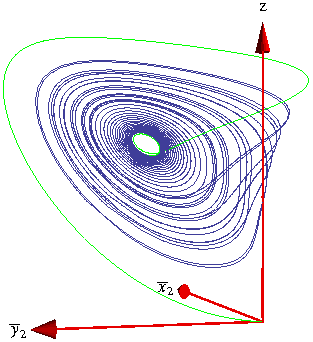
\includegraphics[width=0.35\textwidth,clip=true]{CLEinvXYZ}
~~~~(\textit{b})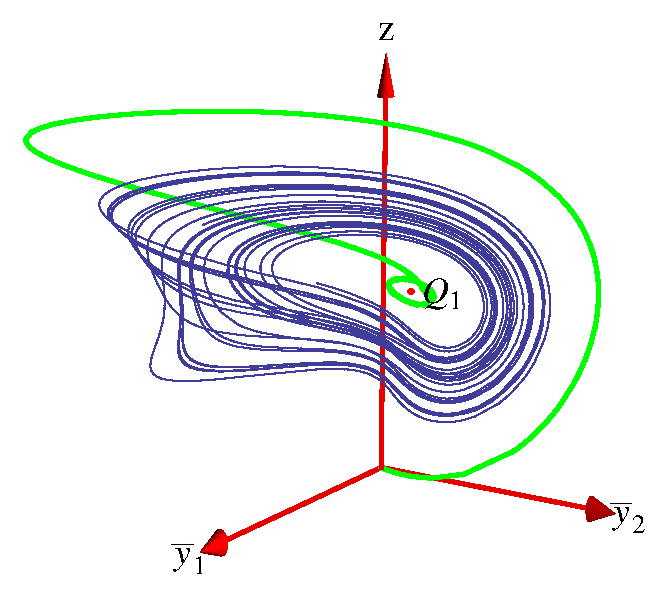
\includegraphics[width=0.35\textwidth,clip=true]{CLEinvYYZ}
\end{center}
\caption{
\Statesp\ portraits of \cLe\ dynamics  in \reducedsp,
projected on invariant coordinates \refeq{eq:invLaser2}.
    }
\label{fig:CLEinv}
\end{figure}
%%%%%%%%%%%%%%%%%%%%%%%%%%%%%%%%%%%%%%%%%%%%%%%%%%%%%%%%%%%%%%%%
\ES{Fetch return map figure using unmodified invariants.}

%%%%%%%%%%%%%%%%%%%%%%%%%%%%%%%%%%%%%%%%%%%%%%%%%%%%%%%%%%%%%%%%%%
\begin{figure}[ht]
\begin{center}
%   (\textit{a})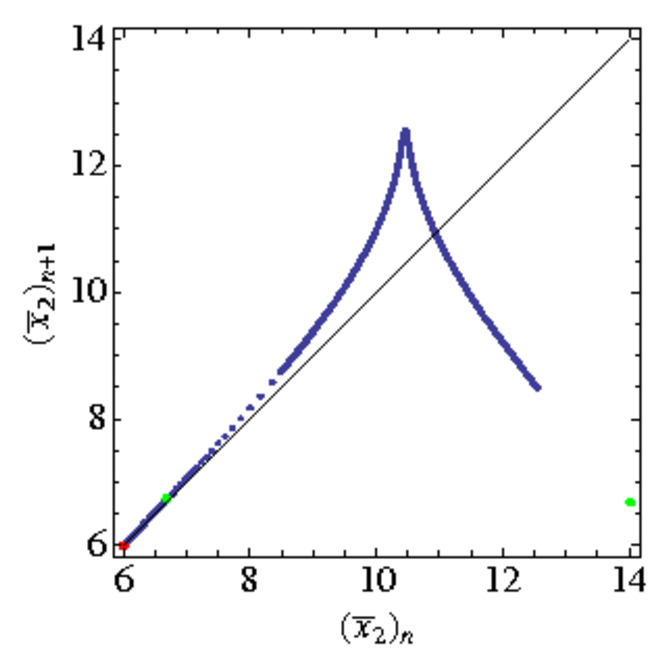
\includegraphics[width=0.35\textwidth,clip=true]{CLEinvRMx2}
%  ~~~~(\textit{b})
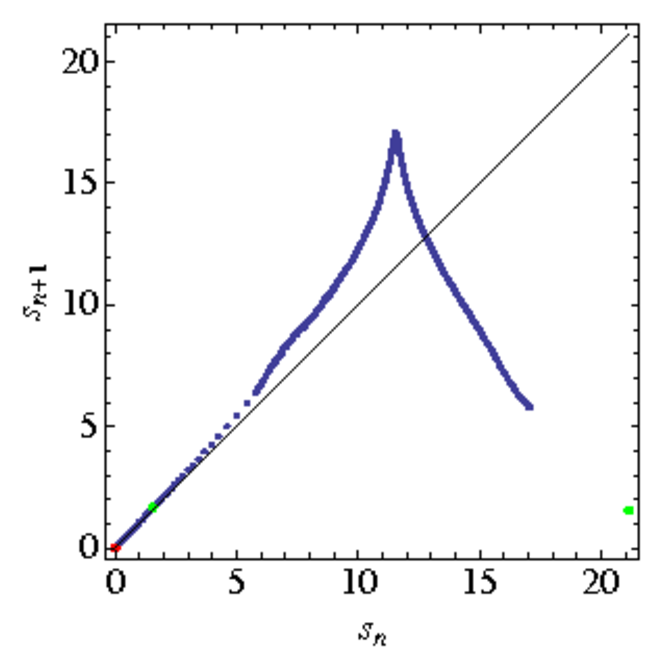
\includegraphics[width=0.35\textwidth,clip=true]{CLEinvRM}
\end{center}
\caption[Return map for Complex Lorenz flow]{
Return map to the \Poincare\ surface of section
$\overline{x}_2=\overline{y}_2$ for \cLe\ with $e=1/10$,
$\ImrCLor=0$, projecting on invariants given in
\refeq{eq:invLaser2}. The return map coordinate is the
Euclidean length along the \Poincare\ section of the unstable
manifold of $E_1$.
    }
\label{fig:CLEinvRM}
\end{figure}
%%%%%%%%%%%%%%%%%%%%%%%%%%%%%%%%%%%%%%%%%%%%%%%%%%%%%%%%%%%%%%%%



